\documentclass{article}
\usepackage{graphicx}
\usepackage{textgreek}
\usepackage[margin=1.5in]{geometry}
\usepackage{indentfirst}

\begin{document}
\title{Spécifiation de conception de la base de données : Jalon 3}

\author{Louis-Vincent CAPELLI \and Alexandre THEISSE \and Tom SARTORI \and Raphaël TURCOTTE}
\date{\today}
\maketitle
\newpage

\tableofcontents
\newpage

\section{Introduction}
\subsection*{Objet et portée du document}
Ce document a pour but de documenter la création d'un entrepôt de données
sur la base de données SSQA et la modification de l'API existante afin de répondre aux 
exigences formulées dans la spécifiation des exigences du modèle pour le jalon 3.
Il s'adresse à toute personne qui pourrait avoir à travailler sur la base de données
SSQA à l'avenir.

\section{Présentation générale du résultat}
Nous avons cloné les schémas \textit{SSQA} et \textit{SSQA\_PUB} correspondants respectivement à
la base de données relationnelle existante et à son API pour obtenir les schémas \textit{SSQA\_2}
et \textit{SSQA\_2\_PUB}. Ces deux groupes de schémas correspondent ainsi à deux bases de données
indépendantes, peuplées avec des données de secteurs différents,
ce qui permet d'émuler l'intégration dans l'entrepôt de données de sources différentes.

Nous avons également créé un nouveau schéma \textit{SSQA\_DIM} qui contient la base de données
dimensionnelle. Ce schéma est peuplé à partir des données de \textit{SSQA} et \textit{SSQA\_2}
par le biais de leur API respective et inclut deux processus celui du déplacement
d'une station et celui de la mesure d'une variable.

\section{Choix de conception}
\subsection{Intégration de plusieurs sources de données}
\subsubsection*{Solution choisie}
Afin de respecter l'exigence d'intégration de plusieurs sources de données, et pour
assurer la compatibilité de celles-ci, nous avons choisi de cloner la base de données
relationnelle existante et son API qui ont été développées lors des jalons précédents.

Chacune des bases de données clonées contenant des données de secteurs différents,
cela permet de mimer l'intégration de deux bases de données distinctes sans avoir à
gérer les problèmes de compatibilité entre celles-ci.

\subsection{Choix des processus à inclure dans l'entrepôt}
\subsubsection*{Solution choisie}
Nous avons choisi d'inclure les processus de déplacement d'une station et 
de mesure d'une variable.

\textbf{Déplacement d'une station :} ce processus prend uniquement 
en compte le déplacement d'une station 
lorsqu'elle est arrêtée et physiquement déplacée d'un point A à un point B. 
Le déplacement continu d'une station mobile qui serait toujours 
en fonctionnement n'est donc pas supporté puisqu'il correspond
selon nous à un autre processus.

Seuls les déplacements terminés sont pris en compte, c'est-à-dire que
les stations qui sont en cours de déplacement ne sont pas considérées
comme déplacées car c'est un cas particulier qui n'arriverait que
très sporadiquement. Ce choix permet de ne pas avoir à rendre \textit{nullable}
les attributs de position et de date de fin de déplacement.

Voici le schéma de l'étoile correspondant à ce processus :

\begin{figure}[ht]
\centering
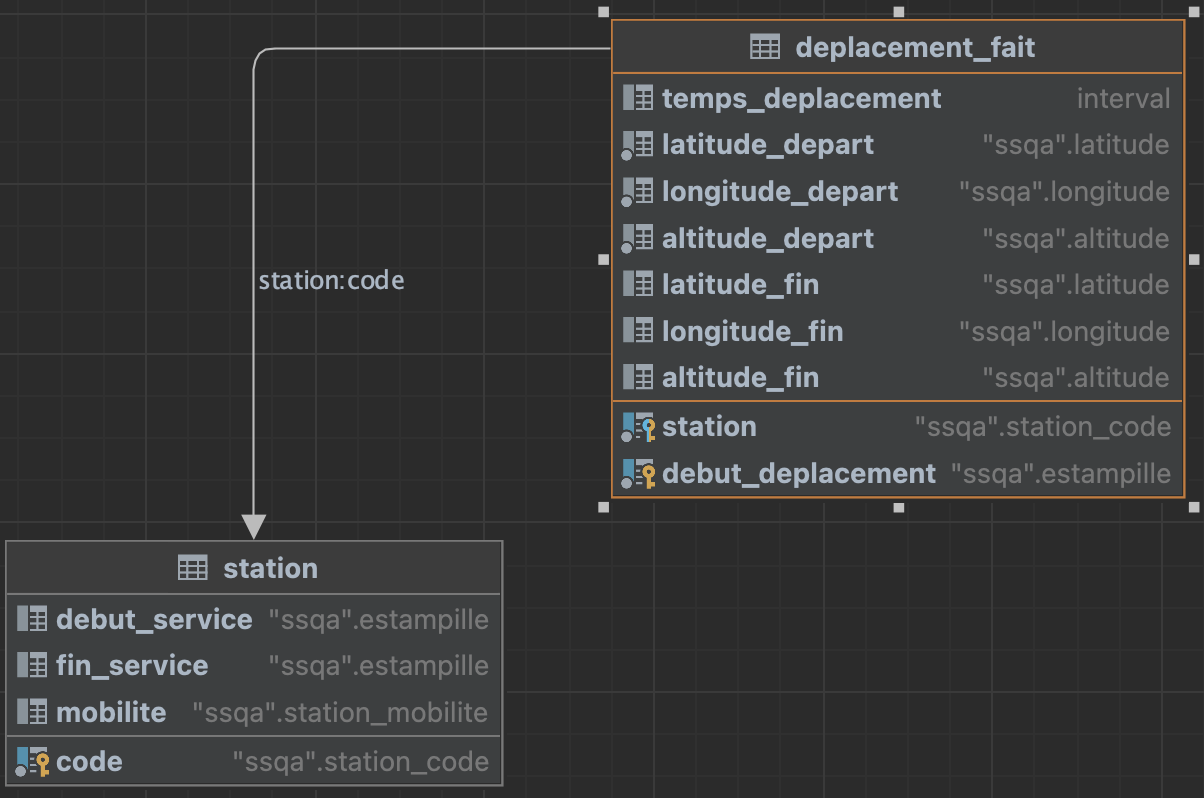
\includegraphics[scale=0.5]{deplacement_fait.png}
\caption{Schéma de l'étoile du processus de déplacement d'une station}
\end{figure}

\textbf{Mesure d'une variable :} nous avons choisi de représenter ce processus
par deux tables de faits distinctes, une pour les mesures valides et l'autre pour
les mesures invalides. 

Cela permet de ne pas avoir à rendre \textit{nullable} les attributs correspondant
aux erreurs (qui n'ont pas lieu d'être dans le cas des mesures valides). De plus,
les mesures invalides sont rarement utilisées conjointement aux mesures valides,
le cas le plus courant étant de vouloir réaliser des statistiques sur l'ensemble
des mesures valides, voire sur l'ensemble des mesures invalides.

Nous avons également inclu dans la table de fait les informations spatio-temporelles
de la station au moment de la mesure afin d'éviter les problèmes de désynchronisation
dans le cas où la station serait déplacée entre la mesure et la consultation de celle-ci.

Voici le schéma de la constellation correspondant à ce processus :

\begin{figure}[ht]
\centering
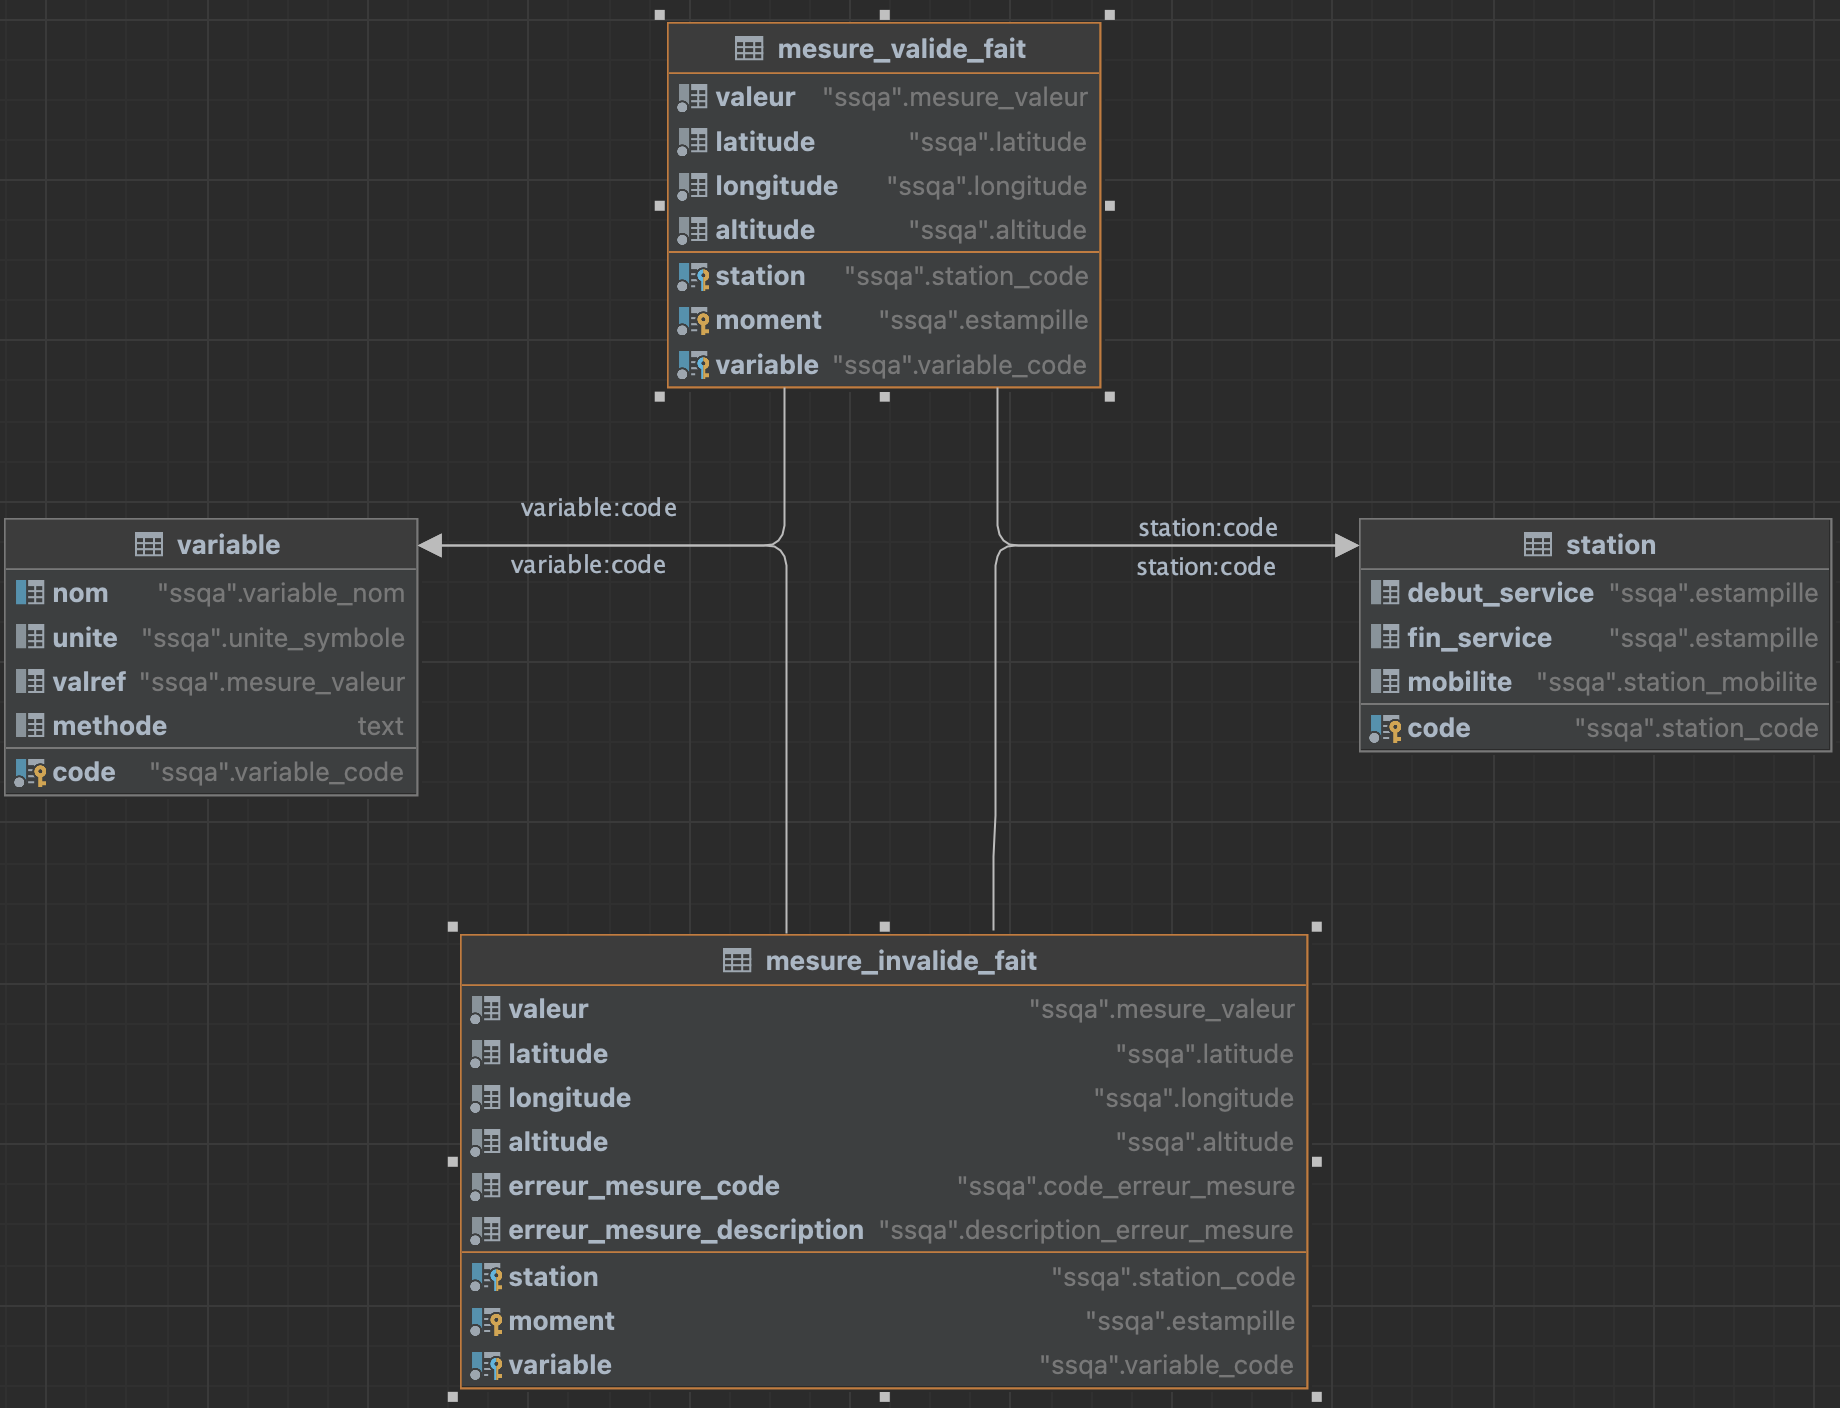
\includegraphics[scale=0.3]{mesure_fait.png}
\caption{Schéma de la constellation du processus de mesure d'une variable}
\end{figure}

\vspace{30cm}
\subsubsection*{Autres Solutions envisagées}
Nous avons réfléchi à une manière d'intégré le processus de l'entretien
du matériel, cependant le schéma de la base de données relationnelle
ne convenait pas. En effet, il ne prend pas en compte les possibles 
interventions nécessaires à la résolution d'un hors-service. Les hors-
service sont donc représentés une date de début et de fin, 
mais aucune information indiquant combien d'interventions ont été nécessaires. 
Dans ce cas, on n'a donc pas de table d'association avec les hors services, 
ni de table d'intervention ce qui rend impossible l'ajout de ce processus.

\subsection{Modifications de l'API}
\subsubsection*{Solution choisie}
Nous avons décidé d'ajouter l'insertion des données dans l'entrepôt aux primitives
ÉMIR de l'API. Dans la plupart des cas, il s'est agit simplement d'ajouter un bloc de code 
dans les primitives d'insertion dans la base de données relationnelle
afin d'insérer également les données dans l'entrepôt.

Le processus de déplacement est un peu particulier : l'insertion d'un déplacement
dans l'entrepôt n'a lieu que lorsque la position d'une station est modifiée dans
la base de données relationnelle. C'est donc la procédure 
$station\_mod\_pos(...)$ (qui permet de modifier les coordonnés d'une station) qui 
s'occupe de l'insertion dans la table de fait du déplacement. Nous avons également
du moodifier la signature de cette procédure car elle partait du principe que la date
de fin d'une position était toujours celle de début de la position suivante, ce qui
ne permet pas de prendre en compte le temps de déplacement. Nous avons donc fait le
choix d'ajouter deux paramètres $i\_fin\_ancienne\_position$ et $i\_debut\_nouvelle\_position$
afin de définir les dates de début et de fin du déplacement.

\subsubsection*{Autres Solutions envisagées}
Nous aurions pu utiliser des after triggers pour effectuer l'insertion dans l'entrepôt
de données mais comme notre API comportait déjà des primitives ÉMIR, leur modification
nous a semblé plus simple et plus propre cohérente avec le reste de l'architecture.

Pour ce qui est de la procédure $station\_mod\_pos(...)$, nous aurions nous passer
du paramètre $i\_debut\_nouvelle\_position$ en utilisant à la place la date actuelle
mais cela aurait signifié que le déplacement d'une station aurait toujours dû être
rentré dans la base de données juste à la fin du déplacement, ce qui nous semblait
peu pratique.

\subsection{Peuplement des bases de données}
\subsubsection*{Solution choisie}
Nous avons choisi de peupler les bases de données à partir de données de secteurs
différents afin de marquer la différence entre les deux sources de données même si
elles présentent le même schéma. Nous avons donc utilisé les données de la ville
Sherbrooke pour la base de données \textit{SSQA} et celles de la ville de Trois-Rivières
pour la base de données \textit{SSQA\_2}.

Ces données ont ainsi été insérées dans les tables de la base de données relationnelle
via leur API respective et donc également dans la base de données dimensionnelle grâce
aux modifications apportées à l'API.

\end{document}
